\section{Eseguire A-CLus Base}

\subsection{Operazioni preliminari}

Prima di poter eseguire il programma, occorre importare il database di A-CLus in MySQL. 

Tale file è presente nella cartella \texttt{A-CLus/Risorse} e si chiama \texttt{mapdb.sql}. 

Per importare il database, è necessario semplciemente accedere al MySQL tramite root e digitare il seguente comando \texttt{source} seguito dal percorso del file \texttt{mapdb.sql}. 

Tale percorso si può ottenere semplicemente trascinando il file del database sul terminale di MySQL.

Alle fine dell'importazione, il terminale di MySQL dovrebbe mostrare un messaggio simile al seguente:

\begin{figure}[h!]
    \centering
    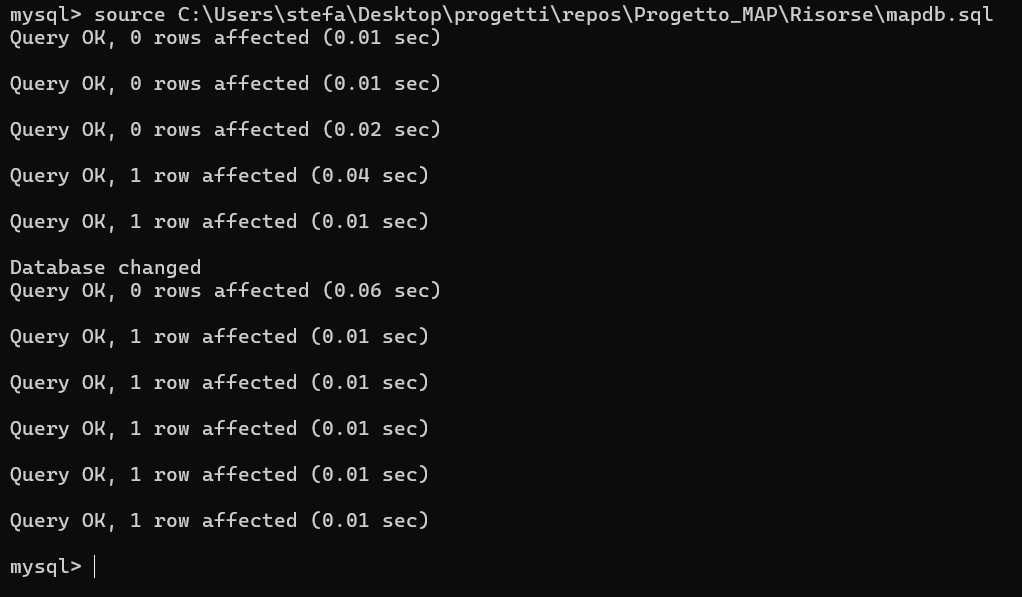
\includegraphics[width=0.5\textwidth]{images/import mysql.png}
\end{figure}

È possibile verificare la corretta importazione anche uscendo da MySQl e accedere con le credenziali dell'utente MapUser, come mostrato nella figura seguente:

\begin{figure}[h!]
    \centering
    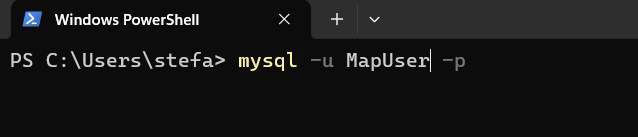
\includegraphics[width=0.5\textwidth]{images/import mapdb.png}
\end{figure}

La password dell'utente MapUser è \texttt{map}. Se viene confermato l'accesso al database, significa che l'importazione è avvenuta con successo. 

\subsection{Avvio dell'applicazione}

Per inizializzare correttamente la versione standard di A-CLus, attenersi alla seguente sequenza operativa:


\begin{enumerate}
    \item Accedere alla directory \texttt{A-CLus\_Base/Bat}
    \item Eseguire il file \texttt{Start\_Server.bat} facendo un doppio click su di esso, assicurandosi che venga mostrato il seguente messaggio a finestra
    
    \begin{figure}[h!]
        \centering
        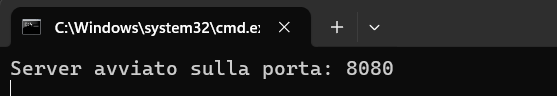
\includegraphics[width=0.5\textwidth]{images/server in esecuzione.png}
    \end{figure}

    \item Dopo aver verificato il corretto funzionamento del server, eseguire il file \texttt{Start\_Client.bat} facendo un doppio click su di esso; se non ci sono problemi con il server, apparirà la seguente schermata:
    
    \begin{figure}[h!]
        \centering
        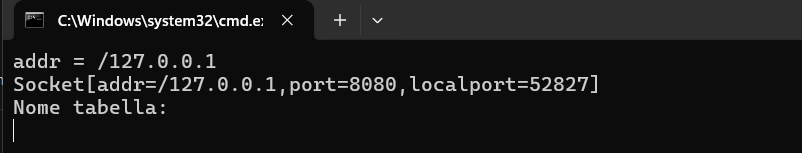
\includegraphics[width=0.5\textwidth]{images/client in esecuzione.png}
        
    \end{figure}
    
\end{enumerate}

\begin{tcolorbox}[colback=white, colframe=gray, title=Avvertenza]
    È necessario mantenere attivo il terminale del server per garantire la comunicazione tra le componenti client e server.
\end{tcolorbox}

\subsection{Avvio dell'ambiente di sviluppo}

Per aprire correttamente il codice sorgente di A-CLus, è necessario seguire le seguenti operazioni nell'ordine in cui sono presentate:

\begin{enumerate}
    \item Aprire la cartella del progetto \texttt{A-CLus\_base}
    \item Incorporare nelle librerie del progetto \texttt{Server} il file \texttt{mySQL\_connector.jar} presente nella cartella \texttt{A-CLus/Risorse}. Nel caso si stia eseguendo il progetto in Visual Studio Code, è possibile eseguire i seguenti passaggi:
    \begin{enumerate}
        \item Aprire il progetto \texttt{A-CLus\_Base}
        \item Recarsi nella sezione \texttt{Referenced Libraries}, in asso a sinistra
        \item Posizionare il cursore sulla cartella e selezionare \texttt{Add JAR/Folder Classpath}, che apparirà sulla destra
        \begin{figure}[h!]
            \centering
            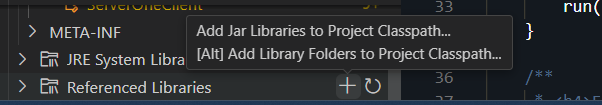
\includegraphics[width=0.5\textwidth]{images/refenereziare il jdbc.png}
        \end{figure}
    \end{enumerate}
    \item Avviare \texttt{MultiServer.java}
    \item Controllare che il server sia in esecuzione correttamente
    \item Aprire il progetto \texttt{MainTest.java} presente nella cartella \texttt{A-CLus\_Base/Client}
\end{enumerate}

\subsection{Interfaccia iniziale}

L'interfaccia iniziale di A-CLus è composta da tre sezioni principali:

\begin{figure}[h!]
    \centering
    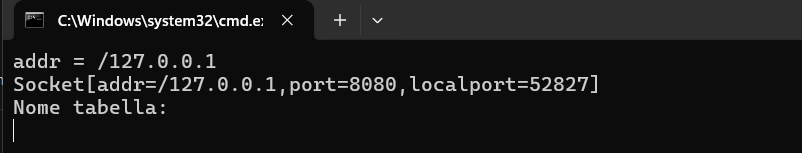
\includegraphics[width=\textwidth]{images/client in esecuzione.png}
    \caption{Interfaccia iniziale di A-CLus}
\end{figure}

L'interfaccia iniziale di A-CLus è composta da tre sezioni principali:

\begin{figure}[h!]
    \centering
    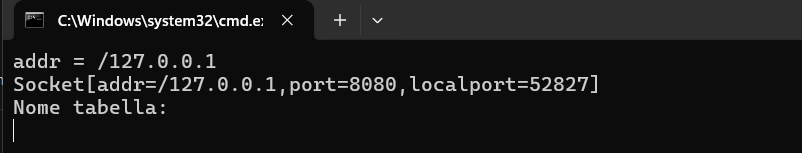
\includegraphics[width=\textwidth]{images/client in esecuzione.png}
    \caption{Interfaccia iniziale di A-CLus}
\end{figure}

\subsection{Selezione delle operazioni disponibili}

\begin{figure}[h!]
    \centering
    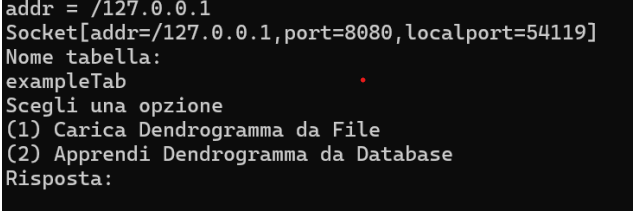
\includegraphics[width=\textwidth]{images/inserimento_tabella.png}
\end{figure}

Dopo l'inserimento della tabella, verrà proposto un menu con due alternative:
\begin{enumerate}
    \item \textbf{Carica Dendrogramma da File}: permette di importare un dendrogramma precedentemente memorizzato
    \item \textbf{Apprendi Dendrogramma da Database}: consente di generare un nuovo dendrogramma analizzando i dati presenti nella tabella selezionata
\end{enumerate}

\subsection{Percorso operativo - Generazione nuovo dendrogramma}

\begin{figure}[h!]
    \centering
    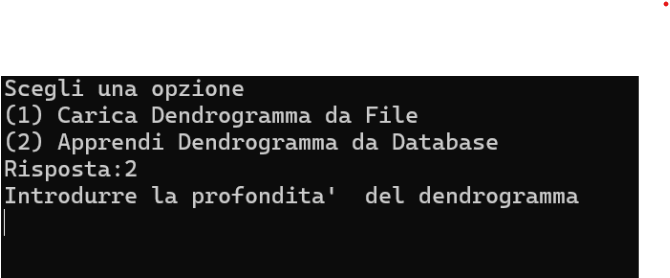
\includegraphics[width=\textwidth]{images/apprendi_datagramma.png}
\end{figure}

Selezionando l'opzione 2, il sistema richiederà l'inserimento del parametro di profondità desiderato per il dendrogramma.

\subsection{Inserimento Profondità}

\begin{figure}[h!]
    \centering
    \includegraphics[width=\textwidth]{images/inserimento_profondità.png}
\end{figure}

Successivamente, l'applicazione proporrà due metodologie di calcolo alternative:
\begin{enumerate}
    \item \textbf{Single-link}: identifica la distanza minima tra cluster, connettendo gli elementi più prossimi tra i gruppi
    \item \textbf{Average-link}: determina la distanza utilizzando la media tra tutti gli elementi dei cluster considerati
\end{enumerate}

\subsubsection{Elaborazione con Single-link}

\begin{figure}[h!]
    \centering
    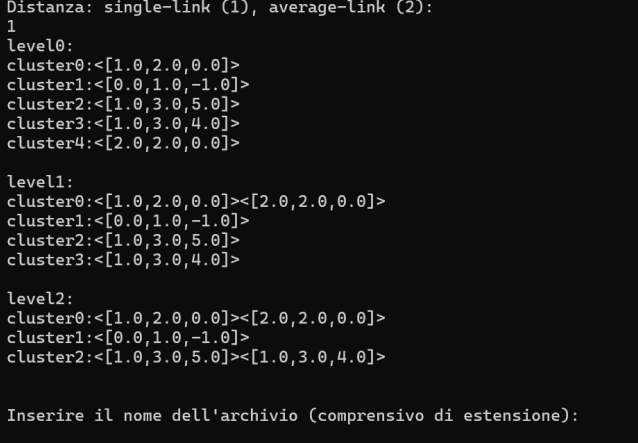
\includegraphics[width=\textwidth]{images/scelta_singleLink.png}
\end{figure}

Selezionando l'opzione Single-link (1), verrà elaborato e visualizzato il dendrogramma risultante. L'applicativo richiederà poi di specificare il nome del file per l'archiviazione del dendrogramma, completo di estensione.

\subsection{Inserimento nome file}

\begin{figure}[h!]
    \centering
    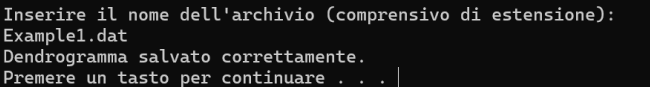
\includegraphics[width=\textwidth]{images/inserimento_nome_file.png}
\end{figure}

Indicare il nome desiderato (esempio: \texttt{Example1.dat}). Il dendrogramma verrà salvato nella cartella \texttt{"saved"} all'interno della directory \texttt{"Jar + Bat"} e l'applicazione terminerà l'esecuzione.

\subsubsection{Elaborazione con Average-link}

\begin{figure}[h!]
    \centering
    \includegraphics[width=\textwidth]{images/scelta_averageLink.png}
\end{figure}

Selezionando l'opzione Average-link (2), il sistema elaborerà il dendrogramma utilizzando il criterio della distanza media e lo visualizzerà a schermo. Successivamente, verrà richiesto di specificare il nome del file per la memorizzazione del dendrogramma, completo di estensione.

\subsection{Percorso operativo - Caricamento dendrogramma esistente}
\begin{figure}[h!]
    \centering
    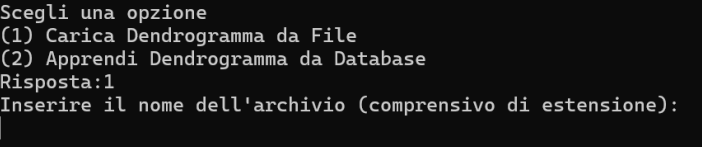
\includegraphics[width=\textwidth]{images/carica_dendrogramma_file.png}
\end{figure}

Selezionando l'opzione 1 per importare un dendrogramma preesistente, sarà necessario indicare il nome completo del file archivio, comprensivo di estensione. I file precedentemente salvati sono localizzati nella cartella \texttt{"saved"} all'interno della directory \texttt{"Jar + Bat"}.

\subsection{Inserimento nome archivio con estensione}

\begin{figure}[h!]
    \centering
    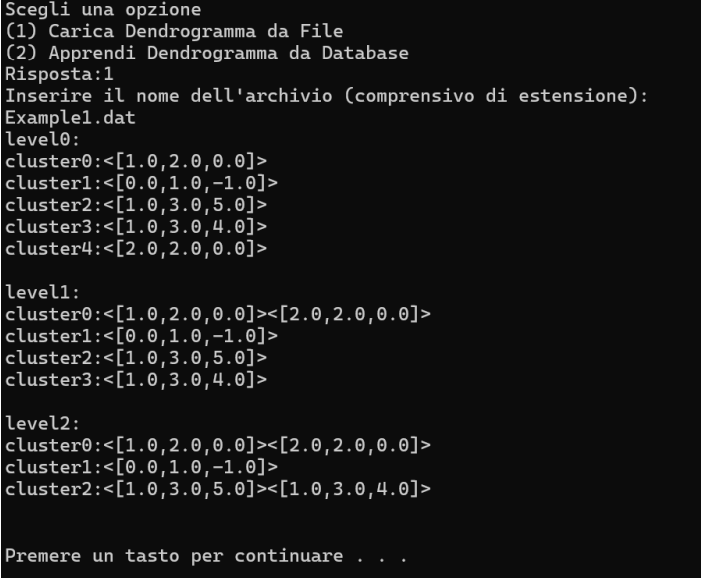
\includegraphics[width=\textwidth]{images/inserimento_nome_archivio.png}
\end{figure}

Dopo l'inserimento del nome dell'archivio, il sistema visualizzerà il dendrogramma caricato e concluderà l'esecuzione.
